%\VignetteIndexEntry{Introduction to the EflowStats package}
%\VignetteEngine{knitr::knitr}
%\VignetteDepends{}
%\VignetteSuggests{xtable}
%\VignetteImports{zoo, XML, RCurl, chron, doBy, hydroGOF, lmomco}
%\VignettePackage{EflowStats}

\documentclass[a4paper,11pt]{article}\usepackage[]{graphicx}\usepackage[]{color}
%% maxwidth is the original width if it is less than linewidth
%% otherwise use linewidth (to make sure the graphics do not exceed the margin)
\makeatletter
\def\maxwidth{ %
  \ifdim\Gin@nat@width>\linewidth
    \linewidth
  \else
    \Gin@nat@width
  \fi
}
\makeatother

\definecolor{fgcolor}{rgb}{0.345, 0.345, 0.345}
\newcommand{\hlnum}[1]{\textcolor[rgb]{0.686,0.059,0.569}{#1}}%
\newcommand{\hlstr}[1]{\textcolor[rgb]{0.192,0.494,0.8}{#1}}%
\newcommand{\hlcom}[1]{\textcolor[rgb]{0.678,0.584,0.686}{\textit{#1}}}%
\newcommand{\hlopt}[1]{\textcolor[rgb]{0,0,0}{#1}}%
\newcommand{\hlstd}[1]{\textcolor[rgb]{0.345,0.345,0.345}{#1}}%
\newcommand{\hlkwa}[1]{\textcolor[rgb]{0.161,0.373,0.58}{\textbf{#1}}}%
\newcommand{\hlkwb}[1]{\textcolor[rgb]{0.69,0.353,0.396}{#1}}%
\newcommand{\hlkwc}[1]{\textcolor[rgb]{0.333,0.667,0.333}{#1}}%
\newcommand{\hlkwd}[1]{\textcolor[rgb]{0.737,0.353,0.396}{\textbf{#1}}}%

\usepackage{framed}
\makeatletter
\newenvironment{kframe}{%
 \def\at@end@of@kframe{}%
 \ifinner\ifhmode%
  \def\at@end@of@kframe{\end{minipage}}%
  \begin{minipage}{\columnwidth}%
 \fi\fi%
 \def\FrameCommand##1{\hskip\@totalleftmargin \hskip-\fboxsep
 \colorbox{shadecolor}{##1}\hskip-\fboxsep
     % There is no \\@totalrightmargin, so:
     \hskip-\linewidth \hskip-\@totalleftmargin \hskip\columnwidth}%
 \MakeFramed {\advance\hsize-\width
   \@totalleftmargin\z@ \linewidth\hsize
   \@setminipage}}%
 {\par\unskip\endMakeFramed%
 \at@end@of@kframe}
\makeatother

\definecolor{shadecolor}{rgb}{.97, .97, .97}
\definecolor{messagecolor}{rgb}{0, 0, 0}
\definecolor{warningcolor}{rgb}{1, 0, 1}
\definecolor{errorcolor}{rgb}{1, 0, 0}
\newenvironment{knitrout}{}{} % an empty environment to be redefined in TeX

\usepackage{alltt}

\usepackage{amsmath}
\usepackage{times}
\usepackage{hyperref}
\usepackage[numbers, round]{natbib}
\usepackage[american]{babel}
\usepackage{authblk}
\usepackage{subfig}
\usepackage{placeins}
\usepackage{footnote}
\usepackage{tabularx}
\usepackage{parskip}
\usepackage{threeparttable}
\usepackage{longtable}
\renewcommand\Affilfont{\itshape\small}

\usepackage{csquotes}
\usepackage{setspace}

\doublespacing

\renewcommand{\topfraction}{0.85}
\renewcommand{\textfraction}{0.1}
\usepackage{graphicx}


\usepackage{mathptmx}% Times Roman font
\usepackage[scaled=.90]{helvet}% Helvetica, served as a model for arial

\usepackage{indentfirst}
\setlength{\parskip}{0pt}

\usepackage{courier}

\usepackage{titlesec}
\usepackage{titletoc}

\titleformat{\section}
  {\normalfont\sffamily\bfseries\LARGE}
  {\thesection}{0.5em}{}
\titleformat{\subsection}
  {\normalfont\sffamily\bfseries\Large}
  {\thesubsection}{0.5em}{}
\titleformat{\subsubsection}
  {\normalfont\sffamily\large}
  {\thesubsubsection}{0.5em}{}
  
\titlecontents{section}
[2.3em]                 % adjust left margin
{\sffamily}             % font formatting
{\contentslabel{2.3em}} % section label and offset
{\hspace*{-2.3em}}
{\titlerule*[0.25pc]{.}\contentspage}
  
\titlecontents{subsection}
[4.6em]                 % adjust left margin
{\sffamily}             % font formatting
{\contentslabel{2.3em}} % section label and offset
{\hspace*{-2.3em}}
{\titlerule*[0.25pc]{.}\contentspage}
  
\titlecontents{subsubsection}
[6.9em]                 % adjust left margin
{\sffamily}             % font formatting
{\contentslabel{2.3em}} % section label and offset
{\hspace*{-2.3em}}
{\titlerule*[0.25pc]{.}\contentspage}

\titlecontents{table}
[0em]                 % adjust left margin
{\sffamily}             % font formatting
{\textbf{Table}\hspace*{2em} \contentslabel {2em}} % section label and offset
{\hspace*{4em}}
{\titlerule*[0.25pc]{.}\contentspage}

\titlecontents{figure}
[0em]                 % adjust left margin
{\sffamily}             % font formatting
{\textbf{Figure}\hspace*{2em} \contentslabel {2em}} % section label and offset
{\hspace*{4em}}
{\titlerule*[0.25pc]{.}\contentspage}

%Italisize and change font of urls:
\urlstyle{sf}
\renewcommand\UrlFont\itshape

\usepackage{caption}
\captionsetup{
  font={sf},
  labelfont={bf,sf},
  labelsep=period,
  justification=justified,
  singlelinecheck=false
}

\setlength\parindent{20pt}

\textwidth=6.5in
\textheight=9in
\parskip=.3cm
\oddsidemargin=.1in
\evensidemargin=.1in
\headheight=-.1in

%------------------------------------------------------------
% newcommand
%------------------------------------------------------------
\newcommand{\scscst}{\scriptscriptstyle}
\newcommand{\scst}{\scriptstyle}
\newcommand{\Robject}[1]{{\texttt{#1}}}
\newcommand{\Rfunction}[1]{{\texttt{#1}}}
\newcommand{\Rclass}[1]{\textit{#1}}
\newcommand{\Rpackage}[1]{\textit{#1}}
\newcommand{\Rexpression}[1]{\texttt{#1}}
\newcommand{\Rmethod}[1]{{\texttt{#1}}}
\newcommand{\Rfunarg}[1]{{\texttt{#1}}}
\IfFileExists{upquote.sty}{\usepackage{upquote}}{}
\begin{document}



\renewenvironment{knitrout}{\begin{singlespace}}{\end{singlespace}}
\renewcommand*\listfigurename{Figures}
\renewcommand*\listtablename{Tables}

%------------------------------------------------------------
\title{The EflowStats R package}
%------------------------------------------------------------
\author[1]{Jessica Thompson}
\author[1]{Stacey Archfield}
\affil[1]{United States Geological Survey}



\noindent{\huge\textsf{\textbf{The EflowStats R package}}}

\noindent\textsf{By Jessica Thompson and Stacey Archfield}

\noindent\textsf{\today}

\tableofcontents
%\listoffigures
\listoftables

%------------------------------------------------------------
\section{Introduction to EflowStats}
%------------------------------------------------------------ 
                
The EflowStats package was created to simplify the process of generating hydrologic indicator statistics using daily streamflow records. It has been specifically designed to work seamlessly with USGS NWIS data, and works with the NWCCompare package to compare USGS National Water Census (\url {http://cida.usgs.gov/nwc/}) modeled and observed streamflow data. This package is intended to be an update of the previously existing USGS NAHAT program \cite{NAHAT} with additional statistics previously published by Archfield et al \cite{Archfield}.     
              
Quantifying the amount of ecologically necessary streamflow and determining the effect of changes in landscape and climate on flow are critical aspects to understanding the ecological health of rivers. A natural flow regime can be characterized using five components of streamflow: magnitude, frequency, duration, timing and rate of change of streamflow. Statistics representing these five properties are commonly applied and the number of ecologically-relevant streamflow statistics (ERSS) available from various software packages is now in the hundreds. The EflowStats package is designed to calculate a comprehensive set of ERSS using the open-source R software environement and provides batch capabilities for calculation of ERSS for multiple sites simultaneously. 

EflowStats also provides the capability to compare two discharge data sets, using direct flow data comparison, as well as frequently used comparison statistics such as Nash-Sutcliffe values, root mean squared error and skewness. This functionality can be used to compared modeled and observed discharge data or two time periods of the same data set. There is a need to examine goodness of fit for surface-water models, and methods differ depending on the intended use of the model. For ecological stream health considerations, the comparison of hydrologic indicator statistics is one judge of fit. The EflowStats package allows for easy comparison of two discharge data sets through direct data comparison and comparison of calculated indices.

EflowStats is both directly available as an R package and integrated into the USGS National Water Census Data Platform. EflowStats will enable easy, transparent and repeatable calculation of many of the most utilized ERSS for many scientists. The EflowStats package is designed to work seamlessly with USGS NWIS web-available data, and users may also load data from other sources (text files, spreadsheets).  Section \ref{sec:exampleWorkflow} provides examples of how one can calculate selected stats from USGS or other data, and how to run data set comparisons. 
              
For information on getting started in R and installing the package, see (\ref{sec:started}): Getting Started.

%------------------------------------------------------------
\section{General Workflow}
\label{sec:exampleWorkflow}
%------------------------------------------------------------ 

This example vignette first loads the relevant packages (assuming they are already installed) and the included sample data. For regular use, you would need to load the packages, but not the given example data.

First, it is a good practice to clear any existing objects from your working environment. In RStudio, in the upper right quadrant, there is a broom icon that says 'Clear'. Click this and select 'Yes' to remove objects. This allows you to being work with a clear workspace, negating the possibility of mis-identified variables. 

\begin{knitrout}
\definecolor{shadecolor}{rgb}{0.969, 0.969, 0.969}\color{fgcolor}\begin{kframe}
\begin{alltt}
\hlkwd{library}\hlstd{(EflowStats)}

\hlcom{############################################}
\hlcom{# Load sample data included with package:}
\hlstd{daily_data}\hlkwb{<-}\hlstd{dailyData}
\end{alltt}
\end{kframe}
\end{knitrout}

To calculate stats for USGS streamgage(s), enter gage id(s), start and end dates and a list of the groups of statistics to be calculated. The list in the example contains all possible statistics.

\begin{knitrout}
\definecolor{shadecolor}{rgb}{0.969, 0.969, 0.969}\color{fgcolor}\begin{kframe}
\begin{alltt}
\hlcom{############################################}
\hlcom{# calculate stats for a USGS streamgage}
\hlstd{sites} \hlkwb{<-} \hlkwd{c}\hlstd{(}\hlstr{"02177000"}\hlstd{,}\hlstr{"02178400"}\hlstd{)}
\hlstd{startdate} \hlkwb{<-} \hlstr{"2009"}
\hlstd{enddate} \hlkwb{<-} \hlstr{"2013"}
\hlstd{stats}\hlkwb{=}\hlstr{"magnifSeven,magStat,flowStat,durStat,timStat,rateStat,otherStat"}
\end{alltt}
\end{kframe}
\end{knitrout}

Once this information is entered, the user runs the ObservedStatsUSGS function and maps the result to a named data frame.



\begin{knitrout}
\definecolor{shadecolor}{rgb}{0.969, 0.969, 0.969}\color{fgcolor}\begin{kframe}
\begin{alltt}
\hlcom{###############################################}
\hlcom{# calculate stats for USGS streamgage(s)}
\hlstd{statsout} \hlkwb{<-} \hlkwd{ObservedStatsUSGS}\hlstd{(sites,startdate,enddate,stats)}
\end{alltt}
\end{kframe}
\end{knitrout}

The retrieved data is now present as a dataframe called 'statsout' in your R environment. This data frame has one row for each gage and one column for each statistic. An example of the first few columns is given below.

\begin{knitrout}
\definecolor{shadecolor}{rgb}{0.969, 0.969, 0.969}\color{fgcolor}\begin{kframe}
\begin{verbatim}
   site_no lam1Obs tau2Obs tau3Obs tau4Obs ar1Obs phaseObs
1 02177000   697.0    0.40    0.31    0.15   0.55    -1.15
2 02178400   190.7    0.39    0.36    0.25   0.47    -1.05
\end{verbatim}
\end{kframe}
\end{knitrout}

This dataframe may now be used within the R environment or saved as a file as shown.

\begin{knitrout}
\definecolor{shadecolor}{rgb}{0.969, 0.969, 0.969}\color{fgcolor}\begin{kframe}
\begin{alltt}
\hlcom{# save statsout to a tab-delimited file}
\hlstd{output} \hlkwb{=} \hlstr{"output.txt"}
\hlkwd{write.table}\hlstd{(statsout,} \hlkwc{file} \hlstd{= output,} \hlkwc{col.names} \hlstd{=} \hlnum{TRUE}\hlstd{,} \hlkwc{row.names} \hlstd{=} \hlnum{FALSE}\hlstd{,}
            \hlkwc{quote} \hlstd{=} \hlnum{FALSE}\hlstd{,} \hlkwc{sep} \hlstd{=} \hlstr{"\textbackslash{}t"}\hlstd{)}
\end{alltt}
\end{kframe}
\end{knitrout}

For daily discharge data not available via NWISWeb, statistics can be calculated by loading data into an R dataframe like the example \texttt{"}dailyData\texttt{"}. This dataframe has two columns, the first named date, containing dates as characters in the format \texttt{"}YYYY-MM-DD\texttt{"} and the second column, discharge, containing the numeric discharge. This can be easily accomplished from most text file formats using \texttt{"}read.delim\texttt{"} or \texttt{"}read.table\texttt{"}. Then the user must enter a drainage area and a site id for each site, as well as the stats string.

\begin{knitrout}
\definecolor{shadecolor}{rgb}{0.969, 0.969, 0.969}\color{fgcolor}\begin{kframe}
\begin{alltt}
\hlcom{#############################################################}
\hlcom{# calculate stats for data from your own data file}
\hlstd{drain_area}\hlkwb{=}\hlnum{54}
\hlstd{site_id}\hlkwb{=}\hlstr{"Test site"}
\hlstd{daily_data}\hlkwb{<-}\hlstd{dailyData}
\hlstd{stats}\hlkwb{=}\hlstr{"magnifSeven,magStat,flowStat,durStat,timStat,rateStat,otherStat"}
\hlstd{statsout} \hlkwb{<-} \hlkwd{ObservedStatsOther}\hlstd{(daily_data,drain_area,site_id,stats)}
\end{alltt}
\end{kframe}
\end{knitrout}

The generated statsout dataframe has the same characteristics as that shown previously. 

The user may wish to generate statistics for a group of sites with locally-stored data. In order to do this, the discharge data must be stored in a local directory, with one file for each site, in the format specified in the previous example. There must also be a file present containing drainage areas for each site, with one column for site number and the second for drainage area. So, for example, the directory may contain 4 files: drainarea.csv, mod02186000.csv, mod02192000.csv and mod02219000.csv, where the files look like the examples shown. 

\begin{table}[ht]
  \begin{threeparttable}[b]
  \caption{drainarea.csv}
  \label{tab:darea}
  \begin{tabularx}{250pt}{|X|X|}
  \hline
\textbf{siteNo} & \textbf{darea} \\ 
  \hline\hline
  02186000 & 106 \\ \hline
  02192000 & 1420 \\ \hline
  02219000 & 176 \\
  \hline
  \end{tabularx}
  \end{threeparttable}
\end{table}

\begin{table}[ht]
  \begin{threeparttable}[b]
  \caption{mod02186000.csv}
  \label{tab:moddata}
  \begin{tabularx}{350pt}{|X|X|X|}
  \hline
\textbf{siteNo} & \textbf{date} & \textbf{discharge} \\ 
  \hline\hline
  02186000 & 1980-10-01 & 4196.27 \\ \hline
  02186000 & 1980-10-02 & 2302.53 \\ \hline
  02186000 & 1980-10-03 & 1202.631 \\ \hline
  02186000 & 1980-10-04 & 863.99 \\ \hline
  02186000 & 1980-10-05 & 709.28 \\ \hline
  02186000 & 1980-10-06 & 637.385 \\
  \hline
  \end{tabularx}
  \end{threeparttable}
\end{table}

\begin{knitrout}
\definecolor{shadecolor}{rgb}{0.969, 0.969, 0.969}\color{fgcolor}\begin{kframe}
\begin{alltt}
\hlcom{###############################################################}
\hlcom{# calculate stats for multiple sites in a local data directory}
\hlstd{dataPath}\hlkwb{=}\hlstr{"C:/Users/jlthomps/Documents/R/JData/modeled/"}
\hlstd{stats}\hlkwb{=}\hlstr{"magnifSeven,magStat,flowStat,durStat,timStat,rateStat,otherStat"}
\hlstd{statsout} \hlkwb{<-} \hlkwd{ObservedStatsOtherMulti}\hlstd{(dataPath,stats)}
\end{alltt}
\end{kframe}
\end{knitrout}

The generated statsout dataframe has the same characteristics as that shown previously.

There is also a function available to plot the monthly means for a daily discharge timeseries. Using included sample data, the following code generates a dataframe of mean monthly discharge and then plots the values with a title containing the site id. 

\begin{knitrout}
\definecolor{shadecolor}{rgb}{0.969, 0.969, 0.969}\color{fgcolor}\begin{kframe}
\begin{alltt}
\hlcom{# plot monthly means for a daily discharge timeseries}
\hlstd{qfiletempf}\hlkwb{<-}\hlstd{sampleData}
\hlstd{meanmonts}\hlkwb{<-}\hlkwd{monthlyMeanTs}\hlstd{(qfiletempf)}
\hlkwd{plotMonthlyMean}\hlstd{(meanmonts,}\hlstr{'02178400'}\hlstd{)}
\end{alltt}
\end{kframe}\begin{figure}[]

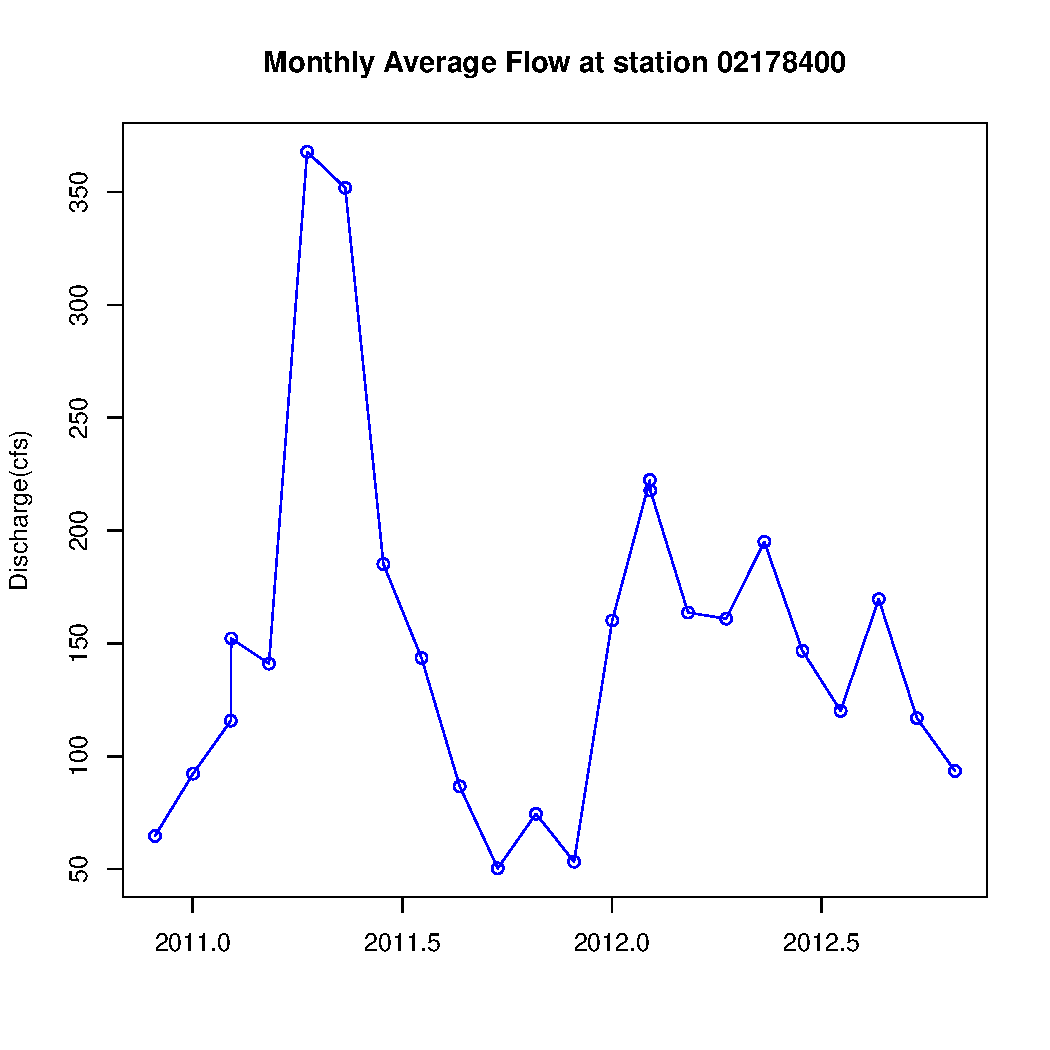
\includegraphics[width=\maxwidth]{figure/plotMonthlyMeans} \caption[Monthly Average Flow at station 02178400]{Monthly Average Flow at station 02178400\label{fig:plotMonthlyMeans}}
\end{figure}


\end{knitrout}

There is one function, CompareStats, that is used to compare the data and calculated statistics for two data sets. It can be used in several ways, three of which are shown here. 

To compare the NWIS observed data for a group of USGS stations with locally stored data (eg modeled data), a list of sites, startDt, endDt, stats string and dataPath are required. The function will then calculate ERSS for each data set, compare the ERSS and directly compare the data sets. These results are then returned in a list (assigned to 'DiffStats' in the example). Statistics for the first data set (the NWIS data) are first in the list, then ERSS for the local data, then ERSS comparison, then ERSS goodness of fit and last the direct data goodness of fit.

\begin{knitrout}
\definecolor{shadecolor}{rgb}{0.969, 0.969, 0.969}\color{fgcolor}\begin{kframe}
\begin{alltt}
\hlcom{#######################################################################}
\hlcom{# NWIS-local}
\hlstd{sites} \hlkwb{<-} \hlkwd{c}\hlstd{(}\hlstr{"02186000"}\hlstd{,}\hlstr{"02192000"}\hlstd{,}\hlstr{"02219000"}\hlstd{,}\hlstr{"02317500"}\hlstd{,}\hlstr{"02329600"}\hlstd{)}
\hlstd{startDt} \hlkwb{<-} \hlstr{"1990"}
\hlstd{endDt} \hlkwb{<-} \hlstr{"1999"}
\hlstd{stats}\hlkwb{=}\hlstr{"magnifSeven,magStat,flowStat,durStat,timStat,rateStat,otherStat"}
\hlstd{dataPath}\hlkwb{=}\hlstr{"C:/Users/jlthomps/Documents/R/JData/modeled/"}
\hlstd{DiffStats} \hlkwb{<-} \hlkwd{CompareStats}\hlstd{(stats,}\hlkwc{sites}\hlstd{=sites,}\hlkwc{dataPath}\hlstd{=dataPath,}\hlkwc{startDt}\hlstd{=startDt,}\hlkwc{endDt}\hlstd{=endDt)}
\hlstd{stats1} \hlkwb{<-} \hlstd{DiffStats[[}\hlnum{1}\hlstd{]]}
\hlstd{stats2} \hlkwb{<-} \hlstd{DiffStats[[}\hlnum{2}\hlstd{]]}
\hlstd{Diffstats} \hlkwb{<-} \hlstd{DiffStats[[}\hlnum{3}\hlstd{]]}
\hlstd{RegGoFstats} \hlkwb{<-} \hlstd{DiffStats[[}\hlnum{4}\hlstd{]]}
\hlstd{GoFstats} \hlkwb{<-} \hlstd{DiffStats[[}\hlnum{5}\hlstd{]]}
\end{alltt}
\end{kframe}
\end{knitrout}

In order to compare data from the same data set, but differing time periods, the CompareStats function requires a list of sites (or dataPath), startDt, endDt, startDt2, endDt2 and the stats string. The function will then return the ERSS for each data set as well as the comparison and goodness of fit of the ERSS. The list returned will not contain the direct data comparison, as there are no matching dates between the two data sets. 

\begin{knitrout}
\definecolor{shadecolor}{rgb}{0.969, 0.969, 0.969}\color{fgcolor}\begin{kframe}
\begin{alltt}
\hlcom{########################################################################}
\hlcom{# NWIS-NWIS}
\hlstd{sites} \hlkwb{<-} \hlkwd{c}\hlstd{(}\hlstr{"02186000"}\hlstd{,}\hlstr{"02192000"}\hlstd{,}\hlstr{"02219000"}\hlstd{,}\hlstr{"02317500"}\hlstd{,}\hlstr{"02329600"}\hlstd{)}
\hlstd{startDt} \hlkwb{<-} \hlstr{"1990"}
\hlstd{endDt} \hlkwb{<-} \hlstr{"1999"}
\hlstd{startDt2} \hlkwb{<-} \hlstr{"2000"}
\hlstd{endDt2} \hlkwb{<-} \hlstr{"2008"}
\hlstd{stats}\hlkwb{=}\hlstr{"magnifSeven,magStat,flowStat,durStat,timStat,rateStat,otherStat"}
\hlstd{DiffStats} \hlkwb{<-} \hlkwd{CompareStats}\hlstd{(stats,}\hlkwc{sites}\hlstd{=sites,}\hlkwc{startDt}\hlstd{=startDt,}\hlkwc{endDt}\hlstd{=endDt,}\hlkwc{startDt2}\hlstd{=startDt2,}\hlkwc{endDt2}\hlstd{=endDt2)}
\end{alltt}
\end{kframe}
\end{knitrout}

In order to compare two locally stored data sets, the CompareStats function requires the stats string, dataPath and dataPath2. Start and end date(s) could be provided if desired. The list returned will contain ERSS for both data sets, the ERSS comparison and goodness of fit and the direct data comparison for any overlapping dates. 

\begin{knitrout}
\definecolor{shadecolor}{rgb}{0.969, 0.969, 0.969}\color{fgcolor}\begin{kframe}
\begin{alltt}
\hlcom{#############################################################################}
\hlcom{# local-local}
\hlstd{stats}\hlkwb{=}\hlstr{"magnifSeven,magStat,flowStat,durStat,timStat,rateStat,otherStat"}
\hlstd{dataPath}\hlkwb{=}\hlstr{"C:/Users/jlthomps/Documents/R/JData/modeled/"}
\hlstd{dataPath2}\hlkwb{=}\hlstr{"C:/Users/jlthomps/Documents/R/JData/observed/"}
\hlstd{DiffStats} \hlkwb{<-} \hlkwd{CompareStats}\hlstd{(stats,}\hlkwc{dataPath}\hlstd{=dataPath,}\hlkwc{dataPath2}\hlstd{=dataPath2)}
\end{alltt}
\end{kframe}
\end{knitrout}

\FloatBarrier

%------------------------------------------------------------
\section{Stats Reference}
\label{sec:reference}
%------------------------------------------------------------

Tables \ref{tab:magStats}, \ref{tab:freqStats}, \ref{tab:durStats}, \ref{tab:timStats}, \ref{tab:rateStats}, \ref{tab:otherStats}, \ref{tab:mag7Stats} and \ref{tab:compStats} summarize the EflowStats functions:

\begin{table}[{|l|X|}[ht]
  \centering
  \begin{threeparttable}[b]
  \caption{EflowStats magnitude functions}
  \label{tab:magStats}
  \begin{tabularx}{\textwidth}{|l|X|}
  \hline
\textbf{Function} & \textbf{Definition} \\ 
  \hline\hline
  ma1 & Mean of the daily mean flow values for the entire flow record \\
  ma2 & Median of the daily mean flow values for the entire flow record \\
  ma3 & Mean (or median - use preference option) of the coefficients of 
  variation (standard deviation/mean) for each year. Compute the coefficient 
  of variation for each year of daily flows. Compute the mean of the annual 
  coefficients of variation \\
  ma4 & Standard deviation of the percentiles of the logs of the entire flow record divided by the mean of percentiles of the logs. Compute the log(10) of the daily flows for the entire record. Compute the 5th, 10th, 15th, 20th, 25th, 30th, 35th, 40th, 45th, 50th, 55th, 60th, 65th, 70th, 75th, 80th, 85th, 90th and 95th percentiles for the logs of the entire flow record. Percentiles are computed by interpolating between the ordered (ascending) logs of the flow values. Compute the standard deviation and mean for the percentile values. Divide the standard deviation by the mean \\
  ma5 & The skewness of the entire flow record is computed as the mean for the entire flow record (ma1) divided by the median (ma2) for the entire flow record \\
  ma6 & Range in daily flows is the ratio of the 10-percent to 90-percent exceedence values for the entire flow record. Compute the 5-percent to 95-percent exceedence values for the entire flow record. Exceedence is computed by interpolating between the ordered (descending) flow values. Divide the 10-percent exceedence by the 90-percent value \\
  ma7 & Range in daily flows is computed in the same way as ma6 except using the 20-percent and 80-percent exceedence values. Divide the 20-percent exceedence value by the 80-percent value \\
  ma8 & Range in daily flows is computed in the same way as ma6 except using the 25-percent and 75-percent exceedence values. Divide the 25-percent exceedence value by the 75-percent value \\
  ma9 & Spread in daily flows is the ratio of the difference between the 90th and 10th percentile of the logs of the flow data to the log of the median of the entire flow record. Compute the log(10) of the daily flows for the entire record. Compute the 5th, 10th, 15th, 20th, 25th, 30th, 35th, 40th, 45th, 50th, 55th, 60th, 65th, 70th, 75th, 80th, 85th, 90th and 95th percentiles for the logs of the entire flow record. Percentiles are computed by interpolating between the ordered (ascending) logs of the flow values. Compute ma9 as (90th-10th)/log10(ma2) \\
  ma10 & Spread in daily flows is computed in the same way as ma9 except using the 20th and 80th percentiles \\
  ma11 & Spread in daily flows is computed in the same way as ma9 except using the 25th and 75th percentiles. \\
  ma12.23 & Means (or medians - use preference option) of monthly flow values. Compute the means for each month over the entire flow record. For example, ma12 is the mean of all January flow values over the entire record. \\
  ma24.35 & Variability (coefficient of variation) of monthly flow values. Compute the standard deviation for each month in each year over the entire flow record. Divide the standard deviation by the mean for each month. Take the mean (or median - use preference option) of these values for each month across all years. \\
  \hline
  \end{tabularx}
  \end{threeparttable}
\end{table}

\begin{table}[ht]
  \centering
  \begin{threeparttable}[b]
  \caption{EflowStats magnitude functions continued}
  \label{tab:mag2Stats}
  \begin{tabularx}{\textwidth}{|l|X|}
  \hline
\textbf{Function} & \textbf{Definition} \\ 
  \hline
  ma36.40 & Variability and skewness across monthly flows. ma36 - compute the minimum, maximum and mean flows for each month in the entire flow record. ma36 is the maximum monthly flow minus the minimum monthly flow divided by the median monthly flow. ma37 - compute the first (25th percentile) and the third (75th percentile) quartiles. ma37 is the third quartile minus the first quartile divided by the median of the monthly means. ma38 - compute the 10th and 90th percentiles for the monthly means. ma38 is the 90th percentile minus the 10th percentile divided by the median of the monthly means. ma39 - compute the standard deviation for the monthly means. ma39 is the standard deviation times 100 divided by the mean of the monthly means. ma40 - skewness in the monthly flows. ma40 is the mean of the monthly flow means minus the median of the monthly means divided by the median of the monthly means. \\
  ma41.45 & Annual runoff and the variability and skewness across annual flows. ma41 - compute the annual mean daily flows. ma41 is the mean of the annual means divided by the drainage area. ma42 is the maximum annual flow minus the minimum annual flow divided by the median annual flow. ma43 - compute the first (25th percentile) and third (75th percentile) quartiles for the annual means. ma43 is the third quartile minus the first quartile divided by the median of the annual means. ma44 - compute the 10th and 90th percentiles for the annual means. ma44 is the 90th percentile minus the 10th percentile divided by the median of the annual means. ma45 - skewness in the annual flows. ma45 is the mean of the annual flow means minus the median of the annual means divided by the median of the annual means. \\
  ml1.12 & Mean (or median - use preference option) minimum flows for each month across all years. Compute the minimum daily flow for each month over the entire flow record. For example ml1 is the mean of the minimums of all January flow values over the entire record. \\
  ml13 & Variability (coefficient of variation) across minimum monthly flow values. Compute the mean and standard deviation for the minimum monthly flows over the entire flow record. ml13 is the standard deviation times 100 divided by the mean minimum monthly flow for all years. \\
  ml14.16 & Minimum annual flow, low flow index and median annual minimum flow. ml14 - compute the minimum annual flow for each year. ml14 is the mean of the ratios of minimum annual flows to the median flow for each year. ml15 - low flow index. ml15 is the mean of the ratios of minimum annual flows to the mean flow for each year. ml16 - median of annual minimum flows. ml16 is the median of the ratios of minimum annual flows to the median flow for each year. \\ 
  ml17 & Base flow. Compute the mean annual flows. Compute the minimum of a 7-day moving average flow for each year and divide them by the mean annual flow for that year. ml17 is the mean (or median - use preference option) of those ratios. \\
  ml18 & Variability in base flow. Compute the standard deviation for the ratios of 7-day moving average flows to mean annual flows for each year. ml18 is the standard deviation times 100 divided by the mean of the ratios. \\
  ml19 & Base flow. Compute the ratios of the minimum annual flow for each year. ml19 is the mean (or median - use preference option) of these ratios times 100. \\
  ml20 & Base flow. Divide the daily flow record into 5-day blocks. Find the minimum flow for each block. Assign the minimum flow as a base flow for that block if 90 percent of that minimum flow is less than the minimum flows for the blocks on either side. Otherwise, set it to zero. Fill in the zero values using linear interpolation. Compute the total flow for the entire record and total base flow for the entire record. ml20 is the ratio of total base flow to total flow. \\
  ml21 & Variability across annual minimum flows. Compute the mean and standard deviation for the annual minimum flows. ml21 is the standard deviation times 100 divided by the mean. \\
    \hline
  \end{tabularx}
  \end{threeparttable}
\end{table}

\begin{table}[ht]
  \centering
  \begin{threeparttable}[b]
  \caption{EflowStats magnitude functions continued}
  \label{tab:mag3Stats}
  \begin{tabularx}{\textwidth}{|l|X|}
  \hline
\textbf{Function} & \textbf{Definition} \\ 
  \hline
  ml22 & Specific mean annual minimum flow. ml22 is the mean (or median - use preference option) of the annual minimum flows divided by the drainage area. \\
  mh1.12 & Mean (or median - use preference option) maximum flows for each month across all years. Compute the maximum daily flow for each month over the entire flow record. For example, mh1 is the mean of the maximums of all January flow values over the entire record. \\
  mh13 & Variability (coefficient of variation) across maximum monthly flow values. Compute the mean and standard deviation for the maximum monthly flows over the entire flow record. mh13 is the standard deviation times 100 divided by the mean maximum monthly flow for all years. \\
  mh14 & Median of annual maximum flows. Compute the annual maximum flows from monthly maximum flows. Compute the ratio of annual maximum flow to median annual flow for each year. mh14 is the median of these ratios. \\
  mh15.17 & High flow discharge index. mh15 is the 1-percent exceedence value for the entire record divided by the median flow for the entire record. mh16 is the 10-percent exceedence value for the entire record divided by the median flow for the entire record. mh17 is the 25-percent exceedence value for the entire record divided by the median flow for the entire record. \\
  mh18 & Variability across annual maximum flows. Compute the logs (log10) of the maximum annual flows. Find the standard deviation and mean for these values. mh18 is the standard deviation times 100 divided by the mean. \\
  mh19 & Skewness in annual maximum flows. Use the equation: (N2*sum(qm3)-3N*sum(qm)*sum(qm2)+2*sum(qm))3)/(N*(N-1)*(N-2)*stddev3) where N=number of years, qm=log10(annual maximum flows), stddev=standard deviation of the annual maximum flows. \\
  mh20 & Specific mean annual maximum flow. mh20 is the mean (or median - use preference option) of the annual maximum flows divided by the drainage area. \\
  mh21 & High flow volume index. Compute the average volume for flow events above a threshold equal to the median flow for the entire record. mh21 is the average volume divided by the median flow for the entire record. \\
  mh22 & High flow volume. Compute the average volume for flow events above a threshold equal to three times the median flow for the entire record. mh22 is the average volume divided by the median flow for the entire record. \\
  mh23 & High flow volume. Compute the average volume for flow events above a threshold equal to seven times the median flow for the entire record. mh23 is the average volume divided by the median flow for the entire record. \\
  mh24 & High peak flow. Compute the average peak flow value for flow events above a threshold equal to the median flow for the entire record. mh24 is the average peak flow divided by the median flow for the entire record. \\
  mh25 & High peak flow. Compute the average peak flow value for flow events above a threshold equal to three times the median flow for the entire record. mh25 is the average peak flow divided by the median flow for the entire record. \\
  mh26 & High peak flow. Compute the average peak flow value for flow events above a threshold equal to seven times the median flow for the entire record. mh26 is the average peak flow divided by the median flow for the entire record. \\
  mh27 & High peak flow. Compute the average peak flow value for flow events above a threshold equal to the 75th percentile value for the entire flow record. mh27 is the average peak flow divided by the median flow for the entire record. \\
   \hline
  \end{tabularx}
  \end{threeparttable}
\end{table}

\begin{table}[ht]
  \centering
  \begin{threeparttable}[b]
  \caption{EflowStats frequency functions}
  \label{tab:freqStats}
\begin{tabularx}{\textwidth}{|l|X|}
  \hline
\textbf{Function} & \textbf{Definition} \\ 
  \hline
  fl1.2 & Low flood pulse count and variability in pulse count. fl1 - Compute the average number of flow events with flows below a threshold equal to the 25th-percentile value for the entire flow record. fl1 is the average (or median - use preference option) number of events. fl2 - Compute the standard deviation in the annual pulse counts for fl1. fl2 is 100 times the standard deviation divided by the mean pulse count. \\
  fl3 & Frequency of low pulse spells. Compute the average number of flow events with flow below a threshold equal to 5-percent of the mean flow values for the entire flow record. fl3 is the mean (or median - use preference option) number of events. \\
  fh1.2 & High flood pulse count and variability in pulse count. fh1 - Compute the average number of flow events with flows above a threshold equal to the 75th-percentile value for the entire flow record. fh1 is the mean (or median - use preference option) number of events. fh2 - compute the standard deviation in the annual pulse counts for fh1. fh2 is 100 times the standard deviation divided by the mean pulse count. \\
  fh3 & High flood pulse count. Compute the average number of days per year that the flow is above a threshold equal to three times the median flow for the entire record. fh3 is the mean (or median-use preference option) of the annual number of days for all years. \\
  fh & High flood pulse count. Compute the average number of days per year that the flow is above a threshold equal to seven times the median flow for the entire record. fh4 is the mean (or median-use preference option) of the annual number of days for all years. \\
  fh5 & Flood frequency. Compute the average number of flow events with flows above a threshold equal to the median flow value for the entire flow record. fh5 is the mean (or median - use preference option) number of events. \\
  fh6 & Flood frequency. Compute the average number of flow events with flows above a threshold equal to three times the median flow value for the entire flow record. fh6 is the mean (or median - use preference option) number of events. \\
  fh7 & Flood frequency. Compute the average number of flow events with flows above a threshold equal to sevent times the median flow value for the entire flow record. fh7 is the mean (or median - use preference option) number of events. \\
  fh8 & Flood frequency. Compute the average number of flow events with flows above a threshold equal to the 25-percent exceedence value for the entire flow record. fh8 is the mean (or median - use preference option) number of events. \\
  fh9 & Flood frequency. Compute the average number of flow events with flows above a threshold equal to the 75-percent exceedence value for the entire flow record. fh9 is the mean (or median - use preference option) number of events. \\
  fh10 & Flood frequency. Compute the average number of flow events with flows above a threshold equal to the median of the annual minima for the entire flow record. fh10 is the mean (or median - use preference option) number of events. \\
  fh11 & Flood frequency. Compute the average number fo flow events with flows above a threshold equal to flow corresponding to a 1.67-year recurrence interval. fh11 is the mean (or median - use preference option) number of events. \\
   \hline
\end{tabularx}
\end{threeparttable}
\end{table}

\begin{table}[ht]
  \centering
  \begin{threeparttable}[b]
  \caption{EflowStats duration functions}
  \label{tab:durStats}
\begin{tabularx}{\textwidth}{|l|X|}
  \hline
\textbf{Function} & \textbf{Definition} \\ 
  \hline
  dl1 & Annual minimum daily flow. Compute the minimum 1-day average flow for each year. dl1 is the man (or median - use preference option) of these values \\
  dl2 & Annual minimum of 3-day moving average flow. compute the minimum of a 3-day moving average flow for each year. dl2 is the mean (or median - use preference option) of these values. \\
  dl3 & Annual minimum of 7-day moving average flow. Compute the minimum of a 7-day moving average flow for each year. dl3 is the mean (or median - use preference option) of these values. \\
  dl4 & Annual minimum of 30-day moving average flow. Compute the minimum of a 30-day moving average flow for each year. dl4 is the mean (or median - use preference option) of these values. \\
  dl5 & Annual minimum of 90-day moving average flow. Compute the minimum of a 90-day moving average flow for each year. dl5 is the mean (or median - use preference option) of these values. \\
  dl6 & Variability of annual minimum daily average flow. Compute the standard deviation for the minimum daily average flow. dl6 is 100 times the standard deviation divided by the mean. \\
  dl7 & Variability of annual minimum of 3-day moving average flow. Compute the standard deviation for the minimum 3-day moving averages. dl7 is 100 times the standard deviation divided by the mean. \\
  dl8 & Variability of annual minimum of 7-day moving average flow. Compute the standard deviation for the minimum 7-day moving averages. dl8 is 100 times the standard deviation divided by the mean. \\
  dl9 & Variability of annual minimum of 30-day moving average flow. Compute the standard deviation for the minimum 30-day moving averages. dl9 is 100 times the standard deviation divided by the mean. \\
  dl10 & Variability of annual minimum of 90-day moving average flow. Compute the standard deviation for the minimum 90-day moving averages. dl10 is 100 times the standard deviation divided by the mean. \\
  dl11 & Annual minimum daily flow divided by the median for the entire record. Compute the minimum daily flow for each year. dl11 is the mean of these values divided by the median for the entire record. \\
  dl12 & Annual minimum of 7-day moving average flow divided by the median for the entire record. Compute the minimum of a 7-day moving average flow for each year. dl12 is the mean of these values divided by the median for the entire record. \\
  dl13 & Annual minimum of 30-day moving average flow divided by the median for the entire record. Compute the minimum of a 30-day moving average flow for each year. dl13 is the mean of these values divided by the median for the entire record. \\
  dl14 & Low exceedence flows. Compute the 75-percent exceedence values for the entire flow record. dl14 is the exceedence value divided by the median for the entire record. \\
  dl15 & Low exceedence flows. Compute the 90-percent exceedence values for the entire flow record. dl15 is the exceedence value divided by the median for the entire record. \\
  dl16.17 & Low flow pulse duration and variability in low pulse duration. dl16 - Compute the average pulse duratino for each year for flow events below a threshold equal to the 25th-percentile value for the entire flow record. dl16 is the median of the yearly average durations. dl17 - compute the standard deviation for the yearly average low pulse durations. dl17 is 100 times the standard deviation divided by the mean of yearly average low pulse durations. \\
    \hline
  \end{tabularx}
  \end{threeparttable}
\end{table}

\begin{table}[ht]
  \centering
  \begin{threeparttable}[b]
  \caption{EflowStats duration functions continued}
  \label{tab:dur2Stats}
  \begin{tabularx}{\textwidth}{|l|X|}
  \hline
\textbf{Function} & \textbf{Definition} \\ 
  \hline
  dl18 & Number of zero-flow days. Count the number of zero-flow days for the entire flow record. dl18 is the mean (or median - use preference option) annual number of zero flow days. \\
  dl19 & Variability is number of zero-flow days. Compute the standard deviation for the annual number of zero-flow days. dl19 is 100 times the standard deviation divided by the mean annual number of zero-flow days. \\
  dl20 & Number of zero-flow months. Count the number of months in which there was no flow over the entire fow record. \\
  dh1 & Annual maximum daily flow. Compute the maximum of a 1-day moving average flow for each year. dh1 is the mean (or median - use preference option) of these values. \\
  dh2 & Annual maximum of 3-day moving average flows. Compute the maximum of a 3-day moving average flow for each year. dh2 is the mean (or median - use preference option) of these values. \\
  dh3 & Annual maximum of 7-day moving average flows. Compute the maximum of a 7-day moving average flow for each year. dh3 is the mean (or median - use preference option) of these values. \\
  dh4 & Annual maximum of 30-day moving average flows. Compute the maximum of a 30-day moving average flow for each year. dh4 is the mean (or median - use preference option) of these values. \\
  dh5 & Annual maximum of 90-day moving average flows. Compute the maximum of a 90-day moving average flow for each year. dh5 is the mean (or median - use preference option) of these values. \\
  dh6 & Variability of annual maximum daily flows. Compute the standard deviation for the maximum 1-day moving averages. dh6 is 100 times the standard deviation divided by the mean. \\
  dh7 & Variability of annual maximum 3-day moving average flows. Compute the standard deviation for the maximum 3-day moving averages. dh7 is 100 times the standard deviation divided by the mean. \\
  dh8 & Variability of annual maximum 7-day moving average flows. Compute the standard deviation for the maximum 7-day moving averages. dh8 is 100 times the standard deviation divided by the mean. \\
  dh9 & Variability of annual maximum 30-day moving average flows. Compute the standard deviation for the maximum 30-day moving averages. dh9 is 100 times the standard deviation divided by the mean. \\
  dh10 & Variability of annual maximum 90-day moving average flows. Compute the standard deviation for the maximum 90-day moving averages. dh10 is 100 times the standard deviation divided by the mean. \\
  dh11 & Annual maximum of 1-day moving average flows divided by the median for the entire record. Compute the maximum of a 1-day moving average flow for each year. dh11 is the mean of these values divided by the median for the entire record. \\
  dh12 & Annual maximum of 7-day moving average flows divided by the median for the entire record. Compute the maximum of a 7-day moving average flow for each year. dh12 is the mean of these values divided by the median for the entire record. \\
  dh13 & Annual maximum of 30-day moving average flows divided by the median for the entire record. Compute the maximum of a 30-day moving average flow for each year. dh13 is the mean of these values divided by the median for the entire record. \\
      \hline
  \end{tabularx}
  \end{threeparttable}
\end{table}

\begin{table}[ht]
  \centering
  \begin{threeparttable}[b]
  \caption{EflowStats duration functions continued}
  \label{tab:dur3Stats}
  \begin{tabularx}{\textwidth}{|l|X|}
  \hline
\textbf{Function} & \textbf{Definition} \\ 
  \hline
  dh14 & Flood duration. Compute the mean of the mean monthly flow values. Find the 95th percentile for the mean monthly flows. dh14 is the 95th percentile value divided by the mean of the monthly means. \\
  dh15.16 & High flow pulse duration and variability of high flow pulse duration. dh15 - Compute the average duration for flow events with flows above a threshold equal to the 75th percentile value for each year in the flow record. dh15 is the median of the yearly average durations. dh16 - Compute the standard deviation for the yearly average high pulse durations. dh16 is 100 times the standard deviation divided by the mean of the yearly average high pulse durations. \\
  dh17 & High flow duration. Compute the average duration of flow events with flows above a threshold equal to the median flow values for the entire flow record. dh17 is the mean (or median - use preference option) duration of the events. \\
  dh18 & High flow duration. Compute the average duration of flow events with flows above a threshold equal to three times the median flow values for the entire flow record. dh18 is the mean (or median - use preference option) duration of the events. \\
  dh19 & High flow duration. Compute the average duration of flow events with flows above a threshold equal to sevent times the median flow values for the entire flow record. dh19 is the mean (or median - use preference option) duration of the events. \\
  dh20 & High flow duration. Compute the 75th percentile value for the entire flow record. Compute the average duration of flow events with flows above a threshold equal to the 75th percentile value for the median annual flows. dh20 is the mean (or median - use preference option) duration of the events. \\
  dh21 & High flow duration. Compute the 25th percentile value for the entire flow record. Compute the average duration of flow events with flows above a threshold equal to the 25th percentile value for the median annual flows. dh21 is the mean (or median - use preference option) duration of the events. \\
  dh22 & Flood interval. Compute the flood threshold as the flow equivalent for a flood recurrence of 1.67 years. Determine the median number of days between flood events for each year. dh22 is the mean (or median - use preference option) of the yearly median number of days between flood events. \\
  dh23 & Flood duration. Compute the flood threshold as the flow equivalent for a flood recurrence of 1.67 years. Determine the number of days each year that the flow remains above the flood threshold. dh23 is the mean (or median - use preference option) of the number of flood days for years in which floods occur. \\
  dh24 & Flood-free days. Compute the flood threshold as the flow equivalent for a flood recurrence of 1.67 years. Compute the maximum number of days that the flow is below the threshold for each year. dh24 is the mean (or median - use preference option) of the maximum yearly no-flood days. \\
   \hline
\end{tabularx}
\end{threeparttable}
\end{table}

\begin{table}[ht]
  \centering
  \begin{threeparttable}[b]
  \caption{EflowStats timing functions}
  \label{tab:timStats}
\begin{tabularx}{\textwidth}{|l|X|}
  \hline
\textbf{Function} & \textbf{Definition} \\ 
  \hline
  ta1.2 & Constancy and predictability. ta1 - Constancy is computed via the formulation of Colwell (see example in Colwell, 1974). A matrix of values is compiled in which the rows are 11 flow categories and the columns are 365 (no February 29th) days of the year. The cell values are the number of times that a flow falls into a category on each day. The row totals, columns totals and grand total are computed. Using the equations for Shannon information theory parameters, constancy is computed as 1 - ((uncertainty with respect to state)/(log10(number of state))). ta2 - predictability is computed from the same matrix as constancy. It is computed as 1 - ((uncertainty with respect to interaction of time and state - uncertainty with respect to time)/(log10(number of state))). \\
  ta3 & Seasonal predictability of flooding. Divide years into 2-month periods (that is, Oct-Nov, Dec-Jan, and so forth). Count the number of flood days (flow events with flows > 1.67-year flood) in each period over the entire flow record. ta3 is the maximum number of flood days in any one period divided by the total number of flood days. \\
  tl1.2 & Julian date of annual minimum and variability in julian date of annual minimum. tl1 - Determine the Julian date that the minimum flow occurs for each water year. Transform the dates to relative values on a circular scale (radians or degrees). Compute the x and y components for each year and average them all across all years. Compute the mean angle as the arc tangent of y-mean divided by x-mean. Transform the resultant angle back to Julian date. tl2 - Compute the coefficient of variation for the mean x and y components and convert to a date. \\
  tl3 & Seasonal predictability of low flow. Divide years into 2-month periods (that is Oct-Nov, Dec-Jan, and so forth). Count the number of low flow events (flow events with flows <= 5-year flood threshold) in each period over the entire flow record. tl3 is the maximum number of low flow events in any one period divided by the total number of low flow events. \\
  tl4 & Seasonal predictability of non-low flow. Compute the number of days that flow is above the 5-year flood threshold as the ratio of number of days to 365 or 366 (leap year) for each year. tl4 is the maximum of the yearly ratios. \\
  th1.2 & Julian date of annual maximum and variability in julian date of annual maximum. th1 - Determine the Julian date that the maximum flow occurs for each year. Transform the dates to relative values on a circular scale (radians or degrees). Compute the x and y components for each year and average them across all years. Compute the mean angle as the arc tangent of y-mean divided by x-mean. Transform the resultant angle back to Julian date. th2 - compute the coefficient of variation for the mean x and y components and convert to a date. \\
  th3 & Seasonal predictability of nonflooding. Computed as the maximum proportion of a 365-day year that the flow is less than the 1.67-year flood threshold and also occurs in all years. Accumulate nonflood days that span all years. th3 is maximum length of those flood-free periods divided by 365. \\
   \hline
\end{tabularx}
\end{threeparttable}
\end{table}

\begin{table}[ht]
  \centering
  \begin{threeparttable}[b]
  \caption{EflowStats rate of change functions}
  \label{tab:rateStats}
\begin{tabularx}{\textwidth}{|l|X|}
  \hline
\textbf{Function} & \textbf{Definition} \\ 
  \hline
  ra1 & Rise rate. Compute the change in flow for days in which the change is positive for the entire flow record. ra1 is the mean (or median - use preference option) of these values. \\
  ra2 & Variability in rise rate. Compute the standard deviation for the positive flow changes. ra2 is 100 times the standard deviation divided by the mean. \\
  ra3 & Fall rate. Compute the change in flow for days in which the change is negative for the entire flow record. ra3 is the mean (or median - use preference option) of these values. \\
  ra4 & Variability in fall rate. Compute the standard deviation for the negative flow changes. ra4 is 100 times the standard deviation divided by the mean. \\
  ra5 & Number of day rises. Compute the number of days in which flow is greater than it was the previous day. ra5 is the number of positive-gain days divided by the total number of days in the flow record. \\
  ra6 & Change of flow. Compute the log10 of the flows for the entire flow record. Compute the change in log of flow for days in which the change is positive for the entire flow record. ra6 is the median of these log values. \\
  ra7 & Change of flow. Compute the log10 of the flows for the entire flow record. Compute the change in log of flow for days in which the change is negative for the entire flow record. ra7 is the median of these log values. \\
  ra8.9 & Number and variability of reversals. ra8 - compute the number of days in each year when the change in flow from one day to the next changes direction. ra8 is the mean (or median - use preference option) of the yearly values. ra9 - compute the standard deviation for the yearly reversal values. ra9 is 100 times the standard deviation divided by the mean. \\
   \hline
\end{tabularx}
\end{threeparttable}
\end{table}

\begin{table}[ht]
  \centering
  \begin{threeparttable}[b]
  \caption{EflowStats other stats functions}
  \label{tab:otherStats}
\begin{tabularx}{\textwidth}{|l|X|}
  \hline
\textbf{Function} & \textbf{Definition} \\ 
  \hline
  mean\_flow & Mean of annual mean discharge values. \\
  med\_flow & Median of annual mean discharge values. \\
  cv\_flow & Coefficient of variation of annual mean discharge values. \\
  cv\_daily & Coefficient of variation of the daily discharge record. \\
  flow\_perc & Flow percentiles of the daily discharge record. Default is 10th, 15th, 25th, 50th, 75th and 90th percentiles, or others can be specified. \\
   \hline
\end{tabularx}
\end{threeparttable}
\end{table}

\begin{table}[ht]
  \centering
  \begin{threeparttable}[b]
  \caption{EflowStats magnificent 7 functions}
  \label{tab:mag7Stats}
\begin{tabularx}{\textwidth}{|l|X|}
  \hline
\textbf{Function} & \textbf{Definition} \\ 
  \hline
  lam1 & Arithmetic mean \\
  tau2 & Coefficient of L-variation - analagous to coefficient of variation. \\
  tau3 & The third L-moment ratio or L-skew. \\
  tau4 & The fourth L-moment ratio or L-kurtosis. \\
  ar1 & AR1 correlation coefficient. \\
  amplitude & Amplitude of the seasonal signal. Compute seasonality variables by first standardizing flows, using the fitting relation A*cos(2*pi*t) + B*sin(2*pi*t). \\
  phase & Phase of the seasonal signal. Compute seasonality variables by first standardizing flows, the fitting relation A*cos(2*pi*t) + B*sin(2*pi*t). \\
   \hline
\end{tabularx}
\end{threeparttable}
\end{table}

\begin{table}[ht]
  \centering
  \begin{threeparttable}[b]
  \caption{EflowStats comparison functions}
  \label{tab:compStats}
\begin{tabularx}{\textwidth}{|l|X|}
  \hline
\textbf{Function} & \textbf{Definition} \\ 
  \hline
  nse & Nash-Sutcliffe value between two data series. \\
  nselog & Nash-Sutcliffe value between the natural logarithms of two data series, with zeros removed. \\
  rmse & Root-mean square error between two data series. \\
  rmsne & Normalized root-mean square error between two data series. \\
  rsr & Ratio of root-mean square error to standard deviation for two data series. \\
  RegionalGoF & Regional goodness of fit. Function calculates nse, nselog, rmse, pbias (percent bias between two data series), pearson correlation coefficient and spearman correlation coefficient for the two sets of flow statistics (modeled and observed). \\
  SiteGoF & Site goodness of fit. Function calculates nse, nselog, rmse, rmsne, rsr, pbias, pearson and  spearman statistics for the entire data series, for the <=10th, 10-25th, 25-50th, 50-75th, 75-90th and >=90th percentiles, and by month for the entire data series. \\
   \hline
\end{tabularx}
\end{threeparttable}
\end{table}

\FloatBarrier
\clearpage

%------------------------------------------------------------ 
\section{Getting Started in R}
\label{sec:started}
%------------------------------------------------------------ 
This section describes the options for downloading and installing the EflowStats package.

%------------------------------------------------------------
\subsection{New to R?}
%------------------------------------------------------------ 
If you are new to R, you will need to first install the latest version of R, which can be found here: \url{http://www.r-project.org/}. There is also a useful USGS site for R help at \url{http://bwtst.usgs.gov/apps/R/index.html}.

There are many options for running and editing R code, one nice environment to learn R is RStudio. RStudio can be downloaded here: \url{http://rstudio.org/}. Once R and RStudio are installed, the dataRetrieval package needs to be installed as described in the next section.

At any time, you can get information about any function in R by typing a question mark before the functions name.  This will open a file (in RStudio, in the Help window) that describes the function, the required arguments, and provides working examples.

\begin{knitrout}
\definecolor{shadecolor}{rgb}{0.969, 0.969, 0.969}\color{fgcolor}\begin{kframe}
\begin{alltt}
\hlkwd{library}\hlstd{(EflowStats)}
\hlopt{?}\hlstd{mh19}
\end{alltt}
\end{kframe}
\end{knitrout}

To see the raw code for a particular code, type the name of the function:
\begin{knitrout}
\definecolor{shadecolor}{rgb}{0.969, 0.969, 0.969}\color{fgcolor}\begin{kframe}
\begin{alltt}
\hlstd{mh19}
\end{alltt}
\begin{verbatim}
function (x) 
{
    annmax <- aggregate(x$discharge, list(x$wy_val), FUN = max, 
        na.rm = TRUE)
    log_disch <- log10(annmax$x)
    sumq3 <- sum(log_disch^3)
    sumq2 <- sum(log_disch^2)
    sumq <- sum(log_disch)
    num_years <- length(unique(x$wy_val))
    qstd <- sd(log_disch)
    mh19 <- round(((num_years * num_years * sumq3) - (3 * num_years * 
        sumq * sumq2) + (2 * sumq * sumq * sumq))/(num_years * 
        (num_years - 1) * (num_years - 2) * qstd * qstd * qstd), 
        digits = 2)
    return(mh19)
}
<environment: namespace:EflowStats>
\end{verbatim}
\end{kframe}
\end{knitrout}

\FloatBarrier
\clearpage
%------------------------------------------------------------
\subsection{R User: Installing EflowStats}
%------------------------------------------------------------ 
Before installing EflowStats, the supporting packages must be first be installed:

\begin{knitrout}
\definecolor{shadecolor}{rgb}{0.969, 0.969, 0.969}\color{fgcolor}\begin{kframe}
\begin{alltt}
\hlkwd{install.packages}\hlstd{(}\hlkwd{c}\hlstd{(}\hlstr{"zoo"}\hlstd{,}\hlstr{"chron"}\hlstd{,}\hlstr{"doBy"}\hlstd{,}\hlstr{"XML"}\hlstd{,}\hlstr{"hydroGOF"}\hlstd{,}\hlstr{"lmomco"}\hlstd{,}\hlstr{"RCurl"}\hlstd{))}
\hlkwd{install.packages}\hlstd{(}\hlstr{"EflowStats"}\hlstd{,}\hlkwc{repos}\hlstd{=}\hlstr{"http://usgs-r.github.com"}\hlstd{,}\hlkwc{type}\hlstd{=}\hlstr{"source"}\hlstd{)}
\end{alltt}
\end{kframe}
\end{knitrout}

It is a good idea to re-start R after installing the package, especially if installing an updated version. Some users have found it necessary to delete the previous version's package folder before installing newer version of dataRetrieval. If you are experiencing issues after updating a package, trying deleting the package folder - the default location for Windows is something like this: C:/Users/userA/Documents/R/win-library/2.15/dataRetrieval, and the default for a Mac: 
/Users/userA/Library/R/2.15/library/dataRetrieval. Then, re-install the package using the directions above. Moving to CRAN should solve this problem.

After installing the package, you need to open the library each time you re-start R.  This is done with the simple command:
\begin{knitrout}
\definecolor{shadecolor}{rgb}{0.969, 0.969, 0.969}\color{fgcolor}\begin{kframe}
\begin{alltt}
\hlkwd{library}\hlstd{(EflowStats)}
\end{alltt}
\end{kframe}
\end{knitrout}

\clearpage

%------------------------------------------------------------------------------------
% BIBLIO
%------------------------------------------------------------------------------------
\begin{thebibliography}{10}

\bibitem{NAHAT}
Henriksen, J.A., Heasley, J. Kennen, J.G., and Nieswand, S., 2006, Users' manual for the Hydroecological Integrity Assessment Process software (including the New Jersey Assessment Tools): U.S. Geological Survey Open-File Report 2006-1093. 72 p.
\url{http://www.fort.usgs.gov/products/publications/21598/21598.pdf}

\bibitem{Archfield}
Archfield, S.A., J.G. Kennen, D.M. Carlisle, and D.M. Wolock. 2013. An Objective and Parsimonious Approach for Classifying Natural Flow Regimes at a Continental Scale. River Res. Applic. doi: 10.1002/rra.2710
\url{http://onlinelibrary.wiley.com/doi/10.1002/rra.2710/abstract}

\end{thebibliography}

\end{document}

\end{document}
